\documentclass[12pt]{article}
\usepackage{epsfig}
\usepackage{tikz}
\usepackage{mathtools, amsmath, amssymb}
\usepackage{qtree}
\usepackage{array, booktabs}
\usepackage{caption}
%\usepackage[margin=0.75in]{geometry}
\usepackage{amsfonts}\usepackage{hyperref}
\hypersetup{
    colorlinks=true,
    citecolor=blue,
    linkcolor=blue,
    filecolor=blue,      
    urlcolor=blue,
    }
\usetikzlibrary{arrows,shapes,decorations,automata,positioning,backgrounds,petri,tikzmark,calc}
\usepackage[
  authordate,
  backend=biber
]{biblatex-chicago}
\addbibresource{references.bib}

% numeric sets
\newcommand{\Reals}{\mathbb{R}}      % real numbers
\newcommand{\Naturals}{\mathbb{N}}   % natural numbers
\newcommand{\Integers}{\mathbb{Z}}   % integer numbers
\newcommand{\Rationals}{\mathbb{Q}}  % rational numbers
\newcommand{\Complexes}{\mathbb{C}}  % complex numbers

% logic
\newcommand{\yields}{\vdash}         % yields
\newcommand{\proves}{\vdash}         % proves
\newcommand{\then}{\rightarrow}      % implication
\newcommand{\logeq}{\Leftrightarrow} % logically equivalent
% formal logic
\newcommand{\Models}{\vDash}                 % models
\newcommand{\Always}{\Box}                   % always
\newcommand{\Eventually}{\lozenge}           % eventually
\newcommand{\Next}{\mathcal{X}}              % ne[X]t
\newcommand{\Until}{\ \mathcal{U}\ }         % [U]ntil
\newcommand{\Release}{\ \mathcal{R}\ }       % [R]lease
\newcommand{\WeakUntil}{\ \mathcal{W}\ }     % [W]eak until
\newcommand{\MightyRelease}{\ \mathcal{M}\ } % [M]ighty release
\newcommand{\Globally}{\mathcal{G}}          % [G]lobally
\newcommand{\Finally}{\mathcal{F}}           % [F]inally
\newcommand{\ForAllPaths}{\mathcal{A}}       % for [A] paths
\newcommand{\ExistsAPath}{\mathcal{E}}       % exists a path

\newcommand{\overbar}[1]{\mkern 1.5mu\overline{\mkern-1.5mu#1\mkern-1.5mu}\mkern 1.5mu}

\listfiles

\title{\bf
\large CS 407 : Applied Formal Methods \\
\large Project Proposal \\
\large Formal Verification of MESI Cache Coherency}
\author{Luke Marzen}
\date{October 26, 2023}

\renewcommand{\baselinestretch}{1.1}
\renewcommand{\arraystretch}{1.2}
\renewcommand{\dbltopfraction}{0.9}
\renewcommand{\topfraction}{0.9}
\renewcommand{\bottomfraction}{0.9}
\renewcommand{\dblfloatpagefraction}{0.99}
\renewcommand{\floatpagefraction}{0.99}
\renewcommand{\textfraction}{0.01}

\newcommand{\N}{\mathbb{N}}
\newcommand{\strings}{\{0, 1\}^\ast}
\newcommand{\dom}{\text{{\it dom} }}
\newcommand{\range}{\text{{\it range}}}
\newcommand{\sstrings}{\Sigma^\ast}
\newcommand{\pair}[2]{{<}#1,{#2}{>}}
\newcommand{\class}[1]{\mathcal{#1}}


\tikzset{fontscale/.style = {font=\relsize{#1}}}

\tikzstyle{startstop} = [rectangle, rounded corners, 
minimum width=1cm, 
minimum height=1cm,
text centered,
text width=2cm,
draw=black,
font = {\scriptsize},
fill=red!30]

\tikzstyle{io} = [trapezium, 
trapezium stretches=true, % A later addition
trapezium left angle=70, 
trapezium right angle=110,
minimum width=1cm, 
minimum height=1cm,
text centered, 
draw=black, fill=blue!30]

\tikzstyle{process} = [rectangle, 
minimum width=1cm, 
minimum height=1cm, 
text centered, 
text width=3cm,
draw=black, 
fill=violet!30]

\tikzstyle{decision} = [diamond, 
minimum width=1cm, 
minimum height=1cm, 
text centered, 
draw=black, 
fill=orange!30]
\tikzstyle{arrow} = [thick,->,>=stealth]


\pagestyle{empty}

\begin{document}

\maketitle

\thispagestyle{empty}


This project is a solo effort by \textit{Luke Marzen}, team \textit{Cache Me Outside}. In modern multi-processor systems, each processor has its own cache used to minimize data access times (Figure \ref{fig:cachediagram}). To maintain a \textit{coherent}, up-to-date, view of shared memory a cache coherency protocol constrains the permitted transactions. One of the most common of these protocols is called MESI. MESI was originally proposed by (\cite{papamarcos1984}) and is named after the four states that a cache-line can be assigned: \textit{Modified}, \textit{Exclusive}, \textit{Shared}, and \textit{Invalid}. The MESI protocol can be defined by a finite-automata shown in Figure \ref{fig:statetransitiondiagram}. Each private cache is connected to a \textit{caching-agent} (i.e. a processor) as well as a bus which monitors all other cache transactions via \textit{Snooping}. Formally, we can define coherency with the following LTL specification (\cite{harrison2010}),

\begin{center}
$\Always \Biggl[
\begin{aligned}
    \forall i.\ &\bigl( \text{Cache}(i) \in \{\texttt{Modified}, \texttt{Exclusive}\} \bigr)\\
    &\then \forall j.\ \bigl( \neg(j = i) \then\ \text{Cache}(j) = \texttt{Invalid} \bigr)
\end{aligned}
\Biggr]$.
\end{center}

\begin{figure}
    \centering
    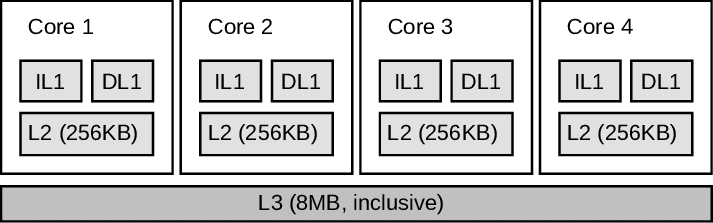
\includegraphics[width=10cm]{images/Intel-Core-i7-cache-architecture.png}
    \caption{Cache architecture of the Intel Core i7 4790 processor. (\cite{nakamoto2018})}
    \label{fig:cachediagram}
\end{figure}

The primary objective of this project is to verify the MESI Cache Coherency Protocol through \textit{Model Checking}. To this end, SPIN will be used to explore the state space and validate that the coherency property is not violated. There are a few additional considerations when creating the model. MESI is modular in the sense that it can be extended beyond the state space of just two caching-agents, with the practical limits being communication overhead and physical footprint of the processor. To verify as many configurations as possible, the number of caching agents $n$ as well as the cache size $m$ will be incremented until the state space becomes too large to model in SPIN. While the size of the caches could vary across caching-agents, in practice it is more common for caches at the same level to be symmetrical. This simplifies creating the model in SPIN and limits the number of configurations. Metrics such as memory usage and execution time of the SPIN verification will recorded so observations can be made about the impacts cache size and number of caching agents. To test that the model correctly represents the protocol, the resulting state space generated by SPIN will be compared to the calculated expected state space for each cache configuration. Furthermore, LTL specifications will be written to further test that each of the allowed transitions can occur, and that no disallowed transitions can occur.
 

\begin{figure}
    \centering
    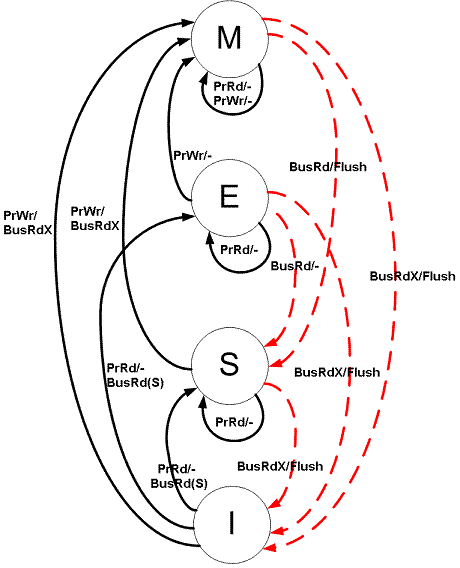
\includegraphics[height=8cm]{images/State_transition_diagram_for_the_Illinois_MESI_protocol.png}
    \caption{State transition diagram for Illinois MESI protocol. Transitions: Processor initiated transactions (black), Bus initiated transaction (red). (\cite{culler1998})}
    \label{fig:statetransitiondiagram}
\end{figure}

The planned timeline is shown in Table \ref{tab:timeline}. Changes will be tracked with git. Work will be done on a development branch, before being later merged into main. The git repository will be structured as follows,
\begin{verbatim}
  applied-formal-methods-final-project-cache-me-outside
  |--reports
  |--models/*.pml
  |--results
\end{verbatim}

\begin{table}[b]
\centering
\captionsetup{labelfont=sc, labelsep=quad}
\caption{Timeline}
\begin{tabular}{@{\,}r <{\hskip 2pt} !{\makebox[0pt]{\textbullet}\hskip-0.5pt\vrule width 1pt\hspace{\labelsep}} >{\raggedright\arraybackslash}p{5cm}}
\toprule
\addlinespace[1.5ex]
Week 10 & Submit Proposal\\
Week 11 & Begin implementing model in SPIN.\\
Week 12 & Prepare for midterm project report/presentation\\
Week 13 & Complete and test model implementation.\\
Thanksgiving Break & --\\
Week 14 & Validate model, gather, and analyze results\\
Week 15 & Prepare for project presentation\\
\end{tabular}
    \label{tab:timeline}
\end{table}



\clearpage{
\printbibliography
}

\end{document}
